% !Mode:: "TeX:UTF-8"	% read in as utf8 file.

\chapter{Math Definitions}
\section{Vector Norm}
$ \ell^2 $-norm (also written "$ l^2 $"-norm) $ |\vec{x}| $ is a \textbf{vector norm} defined for a \textbf{complex vector}

\begin{equation}
\vec{x} = \begin{bmatrix}
x_1 \\ 
x_2 \\ 
\vdots \\ 
x_n
\end{bmatrix} 
\end{equation}

by

\begin{equation}
\label{eq: vector norm defination}
|\vec{x}| = \sqrt{\sum_{k=1}^{n}|x_k|^2}
\end{equation}

where $ |x_k| $ on the right denotes the \textbf{complex modulus}. The $ \ell^2 $-norm is the \textbf{vector norm} that is commonly encountered in vector algebra and vector operations (such as the \textbf{dot product}), where it is commonly denoted $ |\vec{x}| $. However, if desired, a more explicit (but more cumbersome) notation $ |\vec{x}|_2 $ can be used to emphasize the distinction between the \textbf{vector norm} $ |\vec{x}| $ and \textbf{complex modulus} $ |z| $ together with the fact that the $ \ell^2 $-norm is just one of several possible of norms.

For \textbf{real vectors}, the absolute value sign indicating that a complex modulus is being taken on the right of equation \ref{eq: vector norm defination} may be dropped. So, for example, the $ \ell^2 $-norm of the vector $ \vec{x} = (x_1, x_2, x_3) $ is given by

\begin{equation}
|\vec{x}| = \sqrt(x_1^2+x_2^2+x_3^2)
\end{equation}

The $ \ell^2 $-norm is also known as Euclidean norm. However, this is terminology is not recommended since it may cause confusion with the \textbf{Frobenius norm}( a \textbf{matrix norm}) is also sometimes called the Euclidean norm.

The "$ L^2 $-norm" (denoted with an uppercase $ L $) is reserved for application with a function $ \phi(x) $,

\begin{equation}
|\phi|^2 \equiv \phi \cdot \phi \equiv <\phi | \phi> \equiv \int |\phi(x)|^2 dx
\end{equation}

\section{Matrix Norm}
Given a \textbf{square complex} or \textbf{real matrix} $ \mathbf{A} $, a matrix norm $ ||\mathbf{A}|| $ is a \textbf{nonnegative} number associated with $ \mathbf{A} $.

\begin{itemize}
	\item the maximum absolute column sum norm of the matrix
	\begin{equation}
	||\mathbf{A}||_1 = \max\limits_{1 \leq j \leq n} \sum_{i=1}^{m}|a_{ij}|
	\end{equation}
	\item the maximum absolute row sum norm of the matrix
	\begin{equation}
	||\mathbf{A}||_\infty = \max\limits_{1 \leq i \leq m} \sum_{j=1}^{n}|a_{ij}|
	\end{equation}
	\item the \textbf{spectral} norm, which is the square root of the maximum eigenvalue of $ \mathbf{A}^\mathrm{H}\mathbf{A} $, is often referred as "the" matrix norm
	\begin{equation}
	||\mathbf{A}||_2 = \sqrt{\mathrm{maximum~eigenvalue~of~} \mathbf{A}^\mathrm{H}\mathbf{A}}
	\end{equation}
	\item Frobenius norm or $ L_{2,2} $ norm. The equality holds if and only if the matrix $ \mathbf{A} $ is a rank-one matrix or a zero matrix.
	\begin{equation}
	||\mathbf{A}||_F = \sqrt{\sum_{i=1}^{m}\sum_{j=1}^{n}|a_{ij}|^2}
	\end{equation}
\end{itemize}

\subsection{Frobenius Norm}
The Frobenius norm, sometimes also called the Euclidean norm (a term unfortunately also used for the vector $ L^2 $-norm), is \textbf{matrix norm} of an $ m \times n $ matrix $ \mathbf{A} $ defined as the \textbf{square root} of the sum of the absolute squares of its elements,

\begin{equation}
||\mathbf{A}||_F \equiv \sqrt{\sum_{i=1}^{m}\sum_{j=1}^{n}|a_{ij}|^2}
\end{equation}

The Frobenius norm can also be considered as a \textbf{vector norm}.

It is also equal to the \textbf{square root} of the \textbf{matrix trace} of $ \mathbf{AA}^H $, where $ \mathbf{A}^H $ is the conjugate transpose, i.e.,

\begin{equation}
||\mathbf{A}||_F = \sqrt{\mathrm{Tr}(\mathbf{AA}^H)}
\end{equation}

\section{Determinant}
In analytical geometry, determinants express the \textbf{signed volumes of n-dimensional parallelepipeds} .

It can be proven that any matrix has a unique inverse if its determinant is nonzero.

\subsection{$ 2\times 2 $ matrices}
The determinant of a $ 2\times 2 $ matrix is defined by:
\begin{equation}
\det (\mathbf{A}) = \begin{vmatrix}
a & b \\
c & d
\end{vmatrix} = ad-bc
\end{equation}

Supposed a parallelogram defined by two vectors $ \vec{v}_1 = (a,c) $ and $ \vec{v}_2=(b,d) $, so the parallelogram can be expressed with vertices at $ (0,0), (a,b), (a+c, b+d), \mathrm{and~} (c,d) $ as shown in 

\begin{figure}[h]
	\centering
	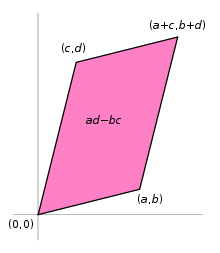
\includegraphics[scale=0.5]{Area_parallellogram_as_determinant}
	\caption{Area parallelogram}
	\label{fig:Area_parallellogram_as_determinant}
\end{figure}

so:
\begin{equation}
\mathrm{Signed~Area} = |\vec{v}_1||\vec{v}_2|\sin \theta = | \vec{v}_1^\bot||\vec{v}_2|\cos \theta' = \begin{bmatrix}
-b \\
a
\end{bmatrix} \cdot \begin{bmatrix}
c \\
d
\end{bmatrix} = ad-bc
\end{equation}

Thus the determinant gives the scaling factor and the orientation induced by the mapping represented by $ \mathbf{A} $. When the determinant is equal to one, the linear mapping defined by the matrix \textbf{equil-area} and \textbf{orientation-preserving}.

\subsection{$ 3\times 3 $ matrices}
The determinant of a $ 3 \times 3 $ matrix (signed volume) is defined by:

\begin{figure}[h]
	\centering
	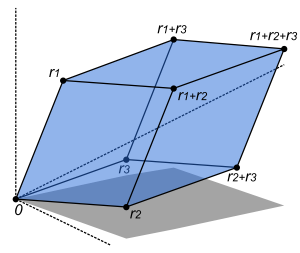
\includegraphics[scale=0.5]{Determinant_parallelepiped}
	\caption{}
	\label{fig:Determinant_parallelepiped}
\end{figure}

\begin{equation}
\begin{split}
\det (\mathbf{A}) &= \begin{vmatrix}
a & b & c\\
d & e & f\\
g & h & i
\end{vmatrix} = a\begin{vmatrix}
e & f\\
h & i
\end{vmatrix}-b\begin{vmatrix}
d & f\\
g & i
\end{vmatrix}+c\begin{vmatrix}
d & e\\
g & h
\end{vmatrix} \\
&= a(ei-fh)-b(di-fg)+c(dh-eg)\\
&= aei+bfg+cdh-ceg-bdi-afh
\end{split}
\end{equation}

\section{Operators}
\subsection{Kronecker product}
In mathematics, the \textbf{Kronecker product}, denoted by $ \otimes $, is an operation on two matrices of arbitrary size resulting in a block matrix. It is generalization of the outer product (which is denoted by the same symbol) from vectors to matrices, and gives the matrix of the tensor product with respect to a standard choice of basis. The Kronecker product should not be confused with the usual matrix multiplication, which is an entirely different operation.

If $ \mathbf{A} $ is an $ m \times n $ matrix and $ \mathbf{B} $ is a $ p \times q $ matrix, then the Kronecker product $ \mathbf{A} \otimes \mathbf{B} $ is the $ mp \times nq $ block matrix:
\begin{equation}
\mathbf{A} \otimes \mathbf{B} = \begin{bmatrix}
a_{11} \mathbf{B} & \cdots & a_{1n} \mathbf{B} \\
\vdots & \ddots & \vdots \\
a_{m1} \mathbf{B} & \cdots & a_{mn} \mathbf{B}
\end{bmatrix}
\end{equation}

more explicitly:
\begin{equation}
\mathbf{A} \otimes \mathbf{B} = \begin{bmatrix}
a_{11} b_{11} & a_{11} b_{12} & \cdots & a_{11} b_{1q} & \cdots & \cdots & a_{1n} b_{11} & a_{1n} b_{12} & \cdots & a_{1n} b_{1q} \\
a_{11} b_{21} & a_{11} b_{22} & \cdots & a_{11} b_{2q} & \cdots & \cdots & a_{1n} b_{21} & a_{1n} b_{22} & \cdots & a_{1n} b_{2q} \\
\vdots & \vdots & \ddots & \vdots & & & \vdots & \vdots & \ddots & \vdots \\
a_{11} b_{p1} & a_{11} b_{p2} & \cdots & a_{11} b_{pq} & \cdots & \cdots & a_{1n} b_{p1} & a_{1n} b_{p2} & \cdots & a_{1n} b_{pq} \\
\vdots & \vdots &  & \vdots & \ddots & & \vdots & \vdots & \ddots & \vdots \\
\vdots & \vdots &  & \vdots & & \ddots & \vdots & \vdots & \ddots & \vdots \\
a_{m1} b_{11} & a_{m1} b_{12} & \cdots & a_{m1} b_{1q} & \cdots & \cdots & a_{mn} b_{11} & a_{mn} b_{12} & \cdots & a_{mn} b_{1q} \\
a_{m1} b_{21} & a_{m1} b_{22} & \cdots & a_{m1} b_{2q} & \cdots & \cdots & a_{mn} b_{21} & a_{mn} b_{22} & \cdots & a_{mn} b_{2q} \\
\vdots & \vdots & \ddots & \vdots & & & \vdots & \vdots & \ddots & \vdots \\
a_{m1} b_{p1} & a_{m1} b_{p2} & \cdots & a_{m1} b_{pq} & \cdots & \cdots & a_{mn} b_{p1} & a_{mn} b_{p2} & \cdots & a_{mn} b_{pq} \\
\end{bmatrix}
\end{equation}

If $ \mathbf{A} $ and $ \mathbf{B} $ represent linear transformations $ \mathbf{v}_1 \rightarrow \mathbf{w}_1 $ and $ \mathbf{v}_2 \rightarrow \mathbf{w}_2 $, respectively, then $ \mathbf{A} \otimes \mathbf{B} $ represents the tensor product of the two maps, $ \mathbf{v}_1 \otimes \mathbf{v}_2 \rightarrow \mathbf{w}_1 \otimes \mathbf{w}_2 $

\textbf{Example}
\begin{equation}
\begin{bmatrix}
1 & 2\\3 & 4
\end{bmatrix} \otimes \begin{bmatrix}
0 & 5\\
6 & 7
\end{bmatrix} = \begin{bmatrix}
1 \cdot 0 & 1 \cdot 5 & 2 \cdot 0 & 2 \cdot 5\\
1 \cdot 6 & 1 \cdot 7 & 2 \cdot 6 & 2 \cdot 7\\
3 \cdot 0 & 3 \cdot 5 & 4 \cdot 0 & 4 \cdot 5\\
3 \cdot 6 & 3 \cdot 7 & 4 \cdot 6 & 4 \cdot 7
\end{bmatrix} = \begin{bmatrix}
0 & 5 & 0 & 10\\
6 & 7 & 12 & 14\\
0 & 15 & 0 & 20\\
18 & 21 & 24 & 28
\end{bmatrix}
\end{equation}

\section{Spline section}
\subsection{B-spline}
In the mathematics subfield of numerical analysis, a \textbf{B-spline}, or \textbf{basis spline}, is a spline function that has minimal support with respect to a given degree, smoothness, and domain partition. Any spline function of given degree can be expressed as a linear combination of B-spline of that degree.

A spline function is a piecewise polynomial function of degree $ <k $ in a variable $ x $. The places where the pieces meet are known as knots. The number of internal knots must be equal to, or greater than $ k-1 $. The key property of spline functions is that they are continuous at the knots. Some derivatives of the spline function may also be continuous, depending on whether the knots are distinct or not.

\textbf{Definition}
\noindent\hrule
A B-spline is a piecewise polynomial function of degree $ <n $ in a variable $ x $. It is defined over a domain $ t_0 \le x \le t_m,~m=n $. The points where $ x = t_j $ are known as knots or break-points. The number of internal knots is equal to the degree of the polynomial if there are no knot multiplicities. The knots must be in ascending order. The number of knots is the minimum for the degree of the B-spline, which has a non-zero vale only in the range between the first and last knot. Each piece of the function is a polynomial of degree $ <n $ between and including adjacent knots. A B-spline is a continuous function at the knots. When all internal knots are distinct its derivatives are also continuous up to the derivative of degree $ n-1 $. If internal knots are coincident at a given value of $ x $, the continuity of derivative order is reduced by 1 for each additional knot.

For any given set of knots, the B-spline is unique, hence the name, B being short for Basis. The usefulness of B-splines lies in the fact that any spline function of order $ n $ on a given set of knots can be expressed as a linear combination of B-splines.

\begin{equation}
S_{n,t}(x) = \sum_{i} \alpha_i B_{i,n}(x)
\end{equation}

This follows from the fact that all pieces have the same continuity properties, within their individual range of support, at the knots.

Expressions for the polynomial pieces can be derived by means of a recursion formula

\begin{align}
B_{i,1}(x) &:= \begin{cases}
1~\mathrm{if}~t_i \le x < t_{i+1}\\
0~~~\mathrm{otherwise}
\end{cases}\\
B_{i,k}(x) &:= \dfrac{x-t_i}{t_{i+k-1}-t_i} B_{i,k-1} (x) + \dfrac{t_{i+k}-x}{t_{i+k}-t_{i+1} B_{i+1,k-1}}(x)
\end{align}

That is, $ B_{j,1}(x) $ is piecewise constant one or zero indicating which knot span $ x $ is in (zero if knot span $ j $ is repeated). The recursion equation is in two parts:

\begin{equation}
\dfrac{x-t_i}{t_{i+k-1} - t_i}
\end{equation}

ramps from zero to one as $ x $ goes from $ t_i $ to $ t_{i+k-1} $ and 

\begin{equation}
\dfrac{t_{i+k}-x}{t_{i+k}-t_{i+1}}
\end{equation}

\subsection{Quartic \& biquartic function}
In mathematics, a \textbf{quartic function}, is a function of the form
\begin{equation}
f(x) = a x^4 + b x^3 + c x^2 + d x + e
\end{equation}

where $ a $ is nonzero, which is defined by a polynomial of degree four, called \textbf{quartic polynomial}.

Sometimes the term \textbf{biquartic} is used instead of \textit{quartic}, but, \textbf{biquartic function} refers to a \textbf{quadratic function} of a aquare ( or, equivalently, to the function defined by a quartic polynomial without terms of odd degree), having the form
\begin{equation}
f(x) = a x^4 + c x^2 + e
\end{equation}

A \textbf{quartic equation}, or equation of the fourth degree, is an equation that equates a quartic polynomial to zero, of the form
\begin{equation}
a x^4 + b x^3 + c x^2 + dx + e = 0
\end{equation}

where $ a \neq 0 $

\subsection{Cubic \& bicubic function}
In mathematics, a \textbf{cubic function} is a function of the form
\begin{equation}
f(x) = a x^3 + b x^2 + c x + d
\end{equation}

where $ a $ is nonzero. In other words, a cubic function is defined by a polynomial of degree three.

Setting $ f(x) = 0 $ produces a \textbf{cubic equation} of the form:
\begin{equation}
a x^3 + b x^2 + c x + d = 0
\end{equation}

Cubic splines can be extended to functions of two or more parameters, in several ways. Bicubic splines are often used to interpolate data on a regular grid, such as \textbf{pixel} values in a digital image. \textbf{Bicubic surface patches}, defined by three bicubic splines, are an essential tool in computer graphics.

\section{Rotation In two dimensions}
In two dimensions, every rotation matrix has the following form,
\begin{equation}
R(\theta) = \begin{bmatrix}
\cos \theta & -\sin \theta\\
\sin \theta & \cos \theta
\end{bmatrix}
\end{equation}

\subsection{Common rotations}
Particularly useful are the matrices for \SI{90}{\degree}, \SI{180}{\degree}, and \SI{270}{\degree} counterclockwise rotation:
\begin{align*}
R(\SI{90}{\degree}) &= \begin{bmatrix}
0 & -1\\
1 & 0
\end{bmatrix}\\
R(\SI{180}{\degree}) &= \begin{bmatrix}
-1 & 0\\
0 & -1
\end{bmatrix}\\
R(\SI{270}{\degree}) &= \begin{bmatrix}
0 & 1\\
-1 & 0
\end{bmatrix}
\end{align*}

\section{Rotation In three dimensions}
A basic rotation (also called elemental rotation) is a rotation about one of the axes of a coordinate system. The following three basic rotation matrices rotate vectors by an angle $ \theta $ about the $ x, y $ or $ z $ axis, in three dimensions, using the \textbf{right hand rule}--which codifies their alternating signs.

\begin{align*}
R_x(\theta) &= \begin{bmatrix}
1 & 0 & 0 \\
0 & \cos \theta & -\sin \theta \\
0 & \sin \theta & \cos \theta
\end{bmatrix}\\
R_y(\theta) &= \begin{bmatrix}
\cos \theta & 0 & \sin \theta\\
0 & 1 & 0 \\
-\sin \theta & 0 & \cos \theta
\end{bmatrix}\\
R_z(\theta) &= \begin{bmatrix}
\cos \theta & -\sin \theta & 0 \\
\sin \theta & \cos \theta & 0 \\
0 & 0 & 1
\end{bmatrix}
\end{align*}

For \textbf{column vectors}, each of these basic vector rotations appears counter-clockwise when the axis about which they occur points toward the observer, the coordinate system is right-handed, and the angle $ \theta $ is positive. $ R_z $, for instance, would rotate toward the $ y $-axis a vector aligned with the $ x $-axis, as can easily be checked by operating with $ R_z $ on vector $ (1, 0, 0) $:
\begin{equation}
R_z(\SI{90}{\degree})\begin{bmatrix}
1\\
0\\
0
\end{bmatrix} = \begin{bmatrix}
\cos \SI{90}{\degree} & -\sin \SI{90}{\degree} & 0\\
\sin \SI{90}{\degree} & \cos \SI{90}{\degree} & 0\\
0 & 0 & 1
\end{bmatrix} \begin{bmatrix}
1\\
0\\
0
\end{bmatrix} = \begin{bmatrix}
0 & -1 & 0\\
1 & 0 & 0\\
0 & 0 & 1
\end{bmatrix} \begin{bmatrix}
1\\
0\\
0
\end{bmatrix} = \begin{bmatrix}
0\\
1\\
0
\end{bmatrix} 
\end{equation}

\section{Laplacian matrix}
In the mathematical field of graph theory, the \textbf{Laplacian matrix}, 
sometimes called \textbf{admittance matrix}, \textbf{Kirchhoff matrix} or \textbf{discrete Laplacian}, 
is a matrix representation of a graph.

\subsection{Laplacian matrix for simple graphs}
Given a simple graph $ G $ with $ n $ vertices, its Laplacian matrix $ \mathbf{L}_{n \times n} $ is defined as:

\begin{equation}
L = D - A
\end{equation}

where $ D $ is the degree matrix and $ A $ is the adjacency matrix of the graph.
Since $ G $ is a simple graph, $ A $ only contains $ 1s $ or $ 0s $ and its diagonal elements are all $ 0s $.
In the case of directed graphs, either the indegree or outdegree might be used, depending on the application.
The elements of $ L $ are given by

\begin{equation}
L_{i,j} := \begin{cases}
\deg(v_i)~~\mathrm{if}~i= j \\
-1 \: \mathrm{if}~i \neq j~\mathrm{and}~v_i~\mathrm{is~adjacent~to}~v_j \\
0~~\mathrm{otherwise}
\end{cases}
\end{equation}

where $ \deg(v_i) $ is the degree of vertex $ i $.

\subsection{Example}
Here is a simple example of a labeled, undirected graph and its Laplacian matrix.

\begin{figure}[h]
\centering
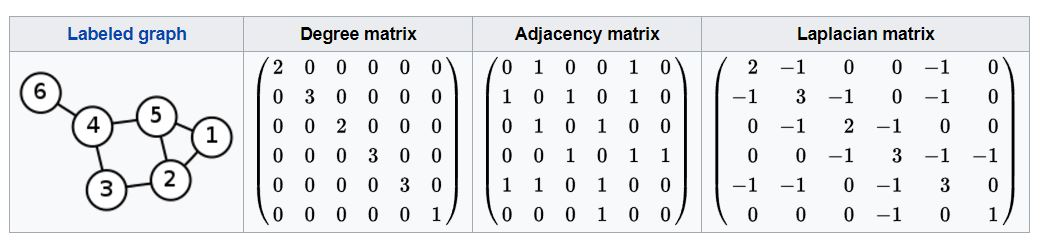
\includegraphics[width=0.8\linewidth]{Figures/example_laplacian_matrix}
\caption{}
\label{fig:example_laplacian_matrix}
\end{figure}
